\documentclass{article}
\usepackage{graphicx, tikz-cd, float, titlepic, booktabs} % Required for inserting images
\usepackage{pgfplots}
\usepackage{multicol}
\usepackage{makecell}
\pgfplotsset{compat=1.9}
\usepackage{mathrsfs}
\usetikzlibrary{arrows}
\usetikzlibrary{decorations.pathreplacing}
\usepackage{amsmath, amssymb, amsthm, amsfonts, siunitx, physics, gensymb}
\AtBeginDocument{\RenewCommandCopy\qty\SI}
\usepackage[version=4]{mhchem}
\usepackage[most,many,breakable]{tcolorbox}
\usepackage{xcolor, fancyhdr, varwidth}
\usepackage[Glenn]{fncychap}
%Options: Sonny, Lenny, Glenn, Conny, Rejne, Bjarne, Bjornstrup
\usepackage{hyperref, cleveref}
\usepackage{icomma, enumitem} %comma as decimal and continue enumerate with [resume]
\usepackage{plimsoll} %use standard state symbol with \stst
\usepackage[danish]{babel}
\renewcommand{\cellalign}{cl}
\renewcommand{\theadalign}{cl}
\renewcommand\theadfont{\bfseries}
\usepackage[round]{natbib} %%Or change 'round' to 'square' for square backers
\usepackage{setspace} %%Enables \doublespacing command for double linespacing
%%%%%%%%%%%%%%%%%%%%%%%%%%%%%%
% SELF MADE COLORS
%%%%%%%%%%%%%%%%%%%%%%%%%%%%%%
\definecolor{myg}{RGB}{56, 140, 70}
\definecolor{myb}{RGB}{45, 111, 177}
\definecolor{myr}{RGB}{199, 68, 64}
\definecolor{mytheorembg}{HTML}{F2F2F9}
\definecolor{mytheoremfr}{HTML}{00007B}
\definecolor{mylenmabg}{HTML}{FFFAF8}
\definecolor{mylenmafr}{HTML}{983b0f}
\definecolor{mypropbg}{HTML}{f2fbfc}
\definecolor{mypropfr}{HTML}{191971}
\definecolor{myexamplebg}{HTML}{F2FBF8}
\definecolor{myexamplefr}{HTML}{88D6D1}
\definecolor{myexampleti}{HTML}{2A7F7F}
\definecolor{mydefinitbg}{HTML}{E5E5FF}
\definecolor{mydefinitfr}{HTML}{3F3FA3}
\definecolor{notesgreen}{RGB}{0,162,0}
\definecolor{myp}{RGB}{197, 92, 212}
\definecolor{mygr}{HTML}{2C3338}
\definecolor{myred}{RGB}{127,0,0}
\definecolor{myyellow}{RGB}{169,121,69}
\definecolor{myexercisebg}{HTML}{F2FBF8}
\definecolor{myexercisefg}{HTML}{88D6D1}
%%%%%%%%%%%%%%%%%%%%%%%%%%%%%%%%%%%%%%%%%%%%%%%%%%%%%%%%%%%%%%%%%%%%%%
% Box environments for theorems and problems
%%%%%%%%%%%%%%%%%%%%%%%%%%%%%%%%%%%%%%%%%%%%%%%%%%%%%%%%%%%%%%%%%%%%%
\setlength{\parindent}{1cm}
%================================
% Question BOX
%================================
\makeatletter
\newtcbtheorem{question}{Opgave}{enhanced,
	breakable,
	colback=white,
	colframe=myb!80!black,
	attach boxed title to top left={yshift*=-\tcboxedtitleheight},
	fonttitle=\bfseries,
	title={#2},
	boxed title size=title,
	boxed title style={%
			sharp corners,
			rounded corners=northwest,
			colback=tcbcolframe,
			boxrule=0pt,
		},
	underlay boxed title={%
			\path[fill=tcbcolframe] (title.south west)--(title.south east)
			to[out=0, in=180] ([xshift=5mm]title.east)--
			(title.center-|frame.east)
			[rounded corners=\kvtcb@arc] |-
			(frame.north) -| cycle;
		},
	#1
}{def}
\makeatother
%================================
% DEFINITION BOX
%================================
\newtheorem{defin}{Definition}[section] % Creates a new counter, number within section

\newtcbtheorem[number within=section, use counter*=defin]{Definition}{Definition}{enhanced,
	before skip=2mm,after skip=2mm, colback=red!5,colframe=red!80!black,boxrule=0.5mm,
	attach boxed title to top left={xshift=1cm,yshift*=1mm-\tcboxedtitleheight}, varwidth boxed title*=-3cm,
	boxed title style={frame code={
					\path[fill=tcbcolback]
					([yshift=-1mm,xshift=-1mm]frame.north west)
					arc[start angle=0,end angle=180,radius=1mm]
					([yshift=-1mm,xshift=1mm]frame.north east)
					arc[start angle=180,end angle=0,radius=1mm];
					\path[left color=tcbcolback!60!black,right color=tcbcolback!60!black,
						middle color=tcbcolback!80!black]
					([xshift=-2mm]frame.north west) -- ([xshift=2mm]frame.north east)
					[rounded corners=1mm]-- ([xshift=1mm,yshift=-1mm]frame.north east)
					-- (frame.south east) -- (frame.south west)
					-- ([xshift=-1mm,yshift=-1mm]frame.north west)
					[sharp corners]-- cycle;
				},interior engine=empty,
		},
	fonttitle=\bfseries,
	title={#2},#1}{def}

\newtcbtheorem[number within=section, use counter*=defin]{definition}{Definition}
{%
	enhanced,
	breakable,
	colback = red!5,
	frame hidden,
	boxrule = 0sp,
	borderline west = {2pt}{0pt}{solid, red!75!black},
	sharp corners,
	detach title,
	before upper = \tcbtitle\par\smallskip,
	coltitle = red!75!black,
	fonttitle = \bfseries\sffamily,
	description font = \mdseries,
	separator sign none,
	segmentation style={solid, red!75!black},
}
{th}

\newtcbtheorem{theo}%
    {Theorem}{}{theorem}
\newtcolorbox{prob}[1]{colback=red!5!white,colframe=red!50!black,fonttitle=\bfseries,title={#1}}
%================================
% NOTE BOX
%================================

\usetikzlibrary{arrows,calc,shadows.blur}
\tcbuselibrary{skins}
\newtcolorbox{note}[1][]{%
	enhanced jigsaw,
	colback=gray!20!white,%
	colframe=gray!80!black,
	size=small,
	boxrule=1pt,
	title=\textbf{Note:},
	halign title=flush center,
	coltitle=black,
	breakable,
	drop shadow=black!50!white,
	attach boxed title to top left={xshift=1cm,yshift=-\tcboxedtitleheight/2,yshifttext=-\tcboxedtitleheight/2},
	minipage boxed title=1.5cm,
	boxed title style={%
			colback=white,
			size=fbox,
			boxrule=1pt,
			boxsep=2pt,
			underlay={%
					\coordinate (dotA) at ($(interior.west) + (-0.5pt,0)$);
					\coordinate (dotB) at ($(interior.east) + (0.5pt,0)$);
					\begin{scope}
						\clip (interior.north west) rectangle ([xshift=3ex]interior.east);
						\filldraw [white, blur shadow={shadow opacity=60, shadow yshift=-.75ex}, rounded corners=2pt] (interior.north west) rectangle (interior.south east);
					\end{scope}
					\begin{scope}[gray!80!black]
						\fill (dotA) circle (2pt);
						\fill (dotB) circle (2pt);
					\end{scope}
				},
		},
	#1,
}
%================================
% EXAMPLE BOX
%================================
\newtcbtheorem[number within=section, use counter from=definition]{example}{Eksempel}
{%
	colback = myexamplebg
	,breakable
	,colframe = myexamplefr
	,coltitle = myexampleti
	,boxrule = 1pt
	,sharp corners
	,detach title
	,before upper=\tcbtitle\par\smallskip
	,fonttitle = \bfseries\sffamily
	,description font = \mdseries
	,separator sign none
}
{ex}
%================================
% THEOREM BOX
%================================

\tcbuselibrary{theorems,skins,hooks}
\newtcbtheorem[number within=section, use counter from=definition]{theorem}{Sætning}
{%
	enhanced,
	breakable,
	colback = mytheorembg,
	frame hidden,
	boxrule = 0sp,
	borderline west = {2pt}{0pt}{mytheoremfr},
	sharp corners,
	detach title,
	before upper = \tcbtitle\par\smallskip,
	coltitle = mytheoremfr,
	fonttitle = \bfseries\sffamily,
	description font = \mdseries,
	separator sign none,
	segmentation style={solid, mytheoremfr},
}
{th}

%%%%%%%%%%%%%%%%%%%%%%%%%%%%%%%%%%%%%%%%%%%%%%%%%%%%%%%%%%%%%%%%%
% SELF MADE COMMANDS
%%%%%%%%%%%%%%%%%%%%%%%%%%%%%%
\newcommand{\sol}{\setlength{\parindent}{0cm}\textbf{\textit{Løsning:}}\setlength{\parindent}{1cm}}
\renewcommand\qedsymbol{$\blacksquare$}
\DeclareMathOperator{\Vm}{Vm}
%%%%%%%%%%%%%%%%%%%%%%%%%%%%%%%%%
\usepackage[tmargin=2cm,rmargin=1in,lmargin=1in,margin=0.85in,bmargin=2cm,footskip=.2in]{geometry}\pagestyle{fancy}
\lhead{Minrui Kevin Zhou 3.b}

\title{SRP}
\author{Kevin Zhou, 2.b}
\date{\today}

\begin{document}
%----------------------------------------------------------------------------------------
%	TITLE PAGE
%----------------------------------------------------------------------------------------

\begin{titlepage} % Suppresses displaying the page number on the title page and the subsequent page counts as page 1
	\newcommand{\HRule}{\rule{\linewidth}{0.5mm}} % Defines a new command for horizontal lines, change thickness here
	
	\center % Centre everything on the page
	
	%------------------------------------------------
	%	Headings
	%------------------------------------------------
	
	\textsc{\LARGE Virum Gymnasium}\\[1.5cm] % Main heading such as the name of your university/college
	
	\textsc{SRP}\\[0.5cm] % Major heading such as course name
	
	\textsc{Matematik}\\[0.5cm] % Minor heading such as course title
	
	%------------------------------------------------
	%	Title
	%------------------------------------------------
	
	\HRule\\[0.4cm]
	
	{\huge\bfseries Riemann-integralet}\\[0.4cm] % Title of your document
	
	\HRule\\[1.5cm]
	
	%------------------------------------------------
	%	Author(s)
	%------------------------------------------------
	
	\begin{minipage}{0.4\textwidth}
		\begin{flushleft}
			\large
			\textit{Forfatter}\\
			 \textsc{Minrui Kevin Zhou} % Your name
		\end{flushleft}
	\end{minipage}
	~
	\begin{minipage}{0.4\textwidth}
		\begin{flushright}
			\large
			\textit{Vejledere}\\
			\textsc{Niels Nørskov Laursen} % Supervisor's name
		\end{flushright}
	\end{minipage}
	
	% If you don't want a supervisor, uncomment the two lines below and comment the code above
	%{\large\textit{Author}}\\
	%John \textsc{Smith} % Your name
	
	%------------------------------------------------
	%	Date
	%------------------------------------------------
	
	\vfill\vfill\vfill % Position the date 3/4 down the remaining page
	
	{\large\today} % Date, change the \today to a set date if you want to be precise
	
	%------------------------------------------------
	%	Logo
	%------------------------------------------------
	
	%\vfill
	
\includegraphics[width=0.3\textwidth]{fig/VG.png}\\[1cm] % Include a department/university logo - this will require the graphicx package
	 
	%----------------------------------------------------------------------------------------
	
	\vfill % Push the date up 1/4 of the remaining page
	
\end{titlepage}

%----------------------------------------------------------------------------------------

\begin{abstract}
  Dette er mit resumé.
\end{abstract}

\tableofcontents
\thispagestyle{empty}
\newpage
\pagenumbering{arabic}
\section{Indledning}
  \label{sec:Indledning}
%Ordnet legeme def
%\begin{definition}[colbacktitle=red!75!black]{Ordnet legeme}{}
%  Et ordnet legeme er et legeme $\mathbb{F}$ med en delmængde $P \subset \mathbb{F}$, kaldet den positive delmængde med egenskaberne:
%  \begin{itemize}
%    \item Hvis $a \in \mathbb{F}$, så $a \in P$ eller $a=0$ eller $-a \in P$. 
%    \item Hvis $a \in P$, så $-a \not\in P$.
%    \item Hvis $a,\,b \in P$, så $a + b \in P$ og $ab \in P$. 
%  \end{itemize}
%\end{definition}

\section{De reele tal}%
\label{sec:De reele tal}
I dette afsnit vil vi først og fremmest undersøge nogle vigtige egenskaber ved $\mathbb{R}$, der er nødvendige for en stringent opbygning af integrationsteorien.
Derefter indfører vi grundlæggende teori om topologi for $\mathbb{R}$, som vi senere skal bruge til at definere kontinuitet samt grænseværdien for en funktion.\footnote{Afsnittet er baseret på \cite{Rudin1976}, s. 3-33. Vi nøjes dog med at kigge på delmængder af $\mathbb{R}$, hvor Rudins bog behandler teorien mere generelt via metriske rum.}

\subsection{Supremum-egenskaben}%
  \label{sub:Supremum-egenskaben}

\begin{definition}[label=def:overtal]{Overtal, undertal, begrænset}{}
  Antag, at $A \subseteq \mathbb{R}$. 
  Hvis der eksisterer $y \in \mathbb{R}$ sådan at $x \leq y$ for alle $x \in A$, så siges $A$ at være opad begrænset, og $y$ kaldes et overtal for $A$. 

  Hvis der eksisterer $z \in \mathbb{R}$ sådan at $x \geq z$ for alle $x \in A$, så siges $A$ at være nedad begrænset, og $z$ kaldes et undertal for $A$. 

  Hvis $A$ både er opad begrænset og nedad begrænset, så kalder vi $A$ begrænset. 
\end{definition}

Imidlertid, kan det også være interessant at kunne sige noget om, hvorvidt et bestemt overtal er det mindste overtal og om et bestemt undertal er det største undertal.

\begin{definition}[label=def:sup]{Supremum, infimum}{}
  Antag, at $A \subseteq \mathbb{R}$. Et element $y \in \mathbb{R}$ kaldes supremum eller mindste overtal af $A$ og betegnes $\sup A$, hvis $y$ har følgende egenskaber:
  \begin{itemize}
    \item $y$ er et overtal for $A$.
    \item $y \leq z$ for alle overtal $z$ af $A$. 
  \end{itemize}
  Et element $\beta \in \mathbb{R}$ kaldes infimum eller største undertal af $A$ og betegnes $\inf A$, hvis $\beta$ har følgende egenskaber:
  \begin{itemize}
    \item $\beta$ er et undertal for $A$.
    \item $\beta \geq \alpha$ for alle undertal $\alpha$ af $A$. 
  \end{itemize}
\end{definition}

\begin{example}[label=exa:supinf]{Supremum og infimum af mængder}{}
  Betragt mængderne
  \[
  A=\{ a \in \mathbb{R}:a \leq 1 \}\quad \text{og} \quad B=\{ b \in \mathbb{R}: b>0 \}. 
  \] 
  Vi har så $\sup A=1$ og $\inf B=0$.
  Derudover er mængden $A$ ikke nedad begrænset og mængden $B$ er ikke opad begrænset. 
\end{example}

Bemærk, at $\sup A \in A$, hvor $\inf B \not\in B$.
Det næste eksempel viser, at en ikke-tom opad begrænset delmængde af $\mathbb{Q}$ kan have supremum, der ikke er i $\mathbb{Q}$. 

\begin{example}[label=exa:supQ]{\footnote{Eksemplet er baseret på \cite{Axler2024}, s. 9} Ikke-tom opad begrænset delmængde af $\mathbb{Q}$ uden supremum i $\mathbb{Q}$ }{}
  Lad
  \[
  A=\{ a \in \mathbb{Q}:a^2<2 \} 
  \] 
Antag, at $q \in \mathbb{Q}$.
Vi vil vise, at $q \neq \sup A$.
Siden $\sqrt{2} $ er irrational, så må vi have $q^2<2$ eller $q^2>2$. 

Hvis $q^2<2$, kan vi finde et element i $A$, der er lidt større end $q$.
Vælg
\[
  \delta=\frac{2-q^2}{5}.
\] 
Siden $q < \abs{\sqrt{2} }<2$ og $0<\delta \leq \frac{2}{5} <1$, så må der gælde, at $2q+\delta<5$. 
Vi har så 
\begin{equation*}
  \begin{split}
    \left(q + \delta \right)^2 &=q^2+\delta^2+2q \delta\\
    &=q^2+\left(2q+\delta \right) \cdot \delta \\
    &<q^2+5 \delta \\
    &=2.
  \end{split}
  \end{equation*}
  Med andre ord er $q + \delta $ altså et element i $A$, og $q \neq \sup A$.  

  Antag nu, at $q^2>0$ og $q>0$ (når $q \leq 0$ er det trivielt, at $q \neq \sup A$). 
  Lad 
  \begin{equation*}
  \begin{split}
   \alpha &=\frac{q^2-2}{2q}\\
  &=\frac{q}{2}-\frac{1}{q}\\
    &<b.
   \end{split}
  \end{equation*}
  Vi har så $0<\alpha <q$, og der gælder 
  \begin{equation*}
  \begin{split}
    \left(q-\alpha \right)^2&=q^2+\alpha ^2 - 2 q \alpha \\
    &<q^2-2q \alpha \\
    &=q^2-(q^2-2)\\
    &=2.
  \end{split}
  \end{equation*}
  Altså er $q- \alpha $ et overtal for $A$, hvilket vil sige, at $q \neq \sup A$. 
  Vi har nu vist, at mængden $A$ ikke har et supremum i $\mathbb{Q}$. 
\end{example}

Eksempel \ref{exa:supQ} motiverer den næste sætning, som vi her ikke vil bevise, da beviset er relativt langt og ikke interessant for vores foretagende.
Sætningen er dog en følge af måden, hvorpå $\mathbb{R}$ er konstrueret.\footnote{$\mathbb{R}$ kan konstrueres fra $\mathbb{Q}$ via Dedekind-snit. \cite{Rudin1976}, s. 17-21}

\begin{theorem}[label=theo:supremum-egenskab]{$\mathbb{R}$ har supremum-egenskaben}{}
  Antag, at $A \in \mathbb{R}$, $A \neq \emptyset$ og $A$ er opad begrænset. 
  Så eksisterer $\sup A \in \mathbb{R}$.
\end{theorem}

Denne egenskab ved $\mathbb{R}$ kaldes for supremum-egenskaben. 
Bemærk, at en alternativ tilgang her kunne være at definere $\mathbb{R}$ ud fra supremum-egenskaben og derefter bevise $\mathbb{R}$'s eksistens ved konstruktion.
Vi vil nu ud fra supremum-egenskaben af $\mathbb{R}$ vise, at $\mathbb{R}$ også må have infimum-egenskaben. 

\begin{theorem}[label=theo:infimum-egenskab]{$\mathbb{R}$ har infimum-egenskaben  }{}
  Antag, at $A \in \mathbb{R}$, $A \neq \emptyset$ og $A$ er nedad begrænset.
  Så eksisterer $\inf A \in \mathbb{R}$.
\end{theorem}
\begin{proof} 
  Lad 
  \[
  B=\{ b \in \mathbb{R} : b \leq a \text{ for alle } a \in A \}.
  \]  
  Så er $B$ mængden af alle undertal for $A$.
  Siden $A$ er nedad begrænset, så er $B$ ikke tom.
  Siden $A \neq \emptyset$, så er $B$ opad begrænset. 
  Fra supremum-egenskaben eksisterer da $\sup B \in \mathbb{R}$. 

  Per definition \ref{def:sup} har vi så, at $\sup B \leq a$ for alle $a \in A$ (fordi alle elementer af $A$ er overtal for $B$). 
  Siden $\sup B$ også er større end eller lig alle undertal for $A$, så må $\sup B=\inf A$. 
\end{proof}

\subsection{Topologi i $\mathbb{R}$}%
  \label{sub:Topologi i R}
Det skal bemærkes, at når vi arbejder med $\mathbb{R}$, så kan ordene \textit{punkt} og \textit{tal} bruges i flæng.
Begge ord referer i dette tilfælde til elementerne i $\mathbb{R}$.
  
\begin{definition}[label=def:omegn]{Omegn}{}
  Antag $p \in \mathbb{R}$. 
  Så er en omegn af et punkt $p$ en mængde 
  \[
  N_r(p)=\{ q \in \mathbb{R}:\abs{q-p} < r \}, \quad \text{ hvor }r \in \mathbb{R}^+. 
  \] 
  Tallet $r$ kaldes for radius af omegnen $N_r(p)$. 
\end{definition}
Med andre ord, er en omegn af et punkt $p$ mængden af alle punkter indenfor en given afstand fra $p$.
Ved en omegn i $\mathbb{R}$ (som vi lige har defineret) er der altså tale om et interval. 
Dette ses illustreret i \cref{fig:omegn}.
\begin{figure}[H]
\begin{center}
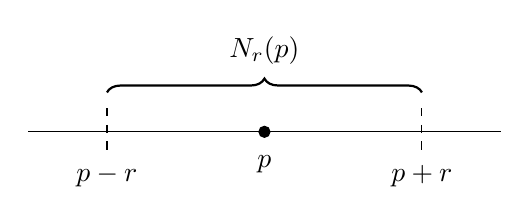
\begin{tikzpicture}
  \centering
    %\tikzstyle{point}=[circle,thick,draw=black,fill=black,inner sep=0pt,minimum width=4pt,minimum height=4pt]
    %\node [point] at (0,0) {};
    \filldraw[black] (0,0) circle (2pt) node[below=5pt]{$p$};
    \draw (-3,0) -- (3,0);
    \draw [dashed] (-2,0.3) -- (-2,-0.3) node[anchor=north]{$p-r$};
    \draw [dashed] (2,0.3) -- (2,-0.3) node[anchor=north]{$p+r$};
    \draw [decorate, decoration = {brace,amplitude=5pt}, thick] (-2,0.5) -- (2,0.5) node[midway,yshift=3.5ex]{$N_r(p)$};
    %\draw [decorate,decoration={brace,amplitude=5pt,mirror,raise=4ex}] (1,0) -- (5,0) node[midway,yshift=-3em]{Konvergenzbereich};
\end{tikzpicture}
\end{center}
  \caption{Illustration af en omegn $N_r(p)$}
\label{fig:omegn}
\end{figure}

\begin{definition}[label=def:åben]{Indre punkt, åben mængde }{}
  Antag, at $A \subseteq \mathbb{R}$. 
  Et punkt $p \in A$ kaldes et indre punkt af $A$, hvis der eksisterer en omegn $N_r(p)$ af $p$ sådan at $N_r(p) \subseteq A$. 

  Mængden $A$ er åben, hvis alle punkter i $A$ er indre punkter. 
\end{definition}

Som eksempel på åbne mængder, kan vi betragte omegne.

\begin{theorem}[label=theo:omegne_åbne]{Omegne er åbne}{}
  Alle omegne $N_r(p)$ af et punkt $p \in \mathbb{R}$ er åbne. 
\end{theorem}
\begin{proof} 
  Lad $q \in N_r(p)$ og $t=r-\abs{p-q} $.
  Så har vi $\abs{p-q} <r$, hvilket vil sige, at $t>0$.
  Fra trekantsuligheden har vi så, at der for alle $s \in N_t(q)$ gælder
  \begin{equation*}
  \begin{split}
    \abs{p-s} &\leq \abs{p-q} + \abs{q-s} \\
    &<\abs{q-p} + t \\
    &=r.
  \end{split}
  \end{equation*}
  Altså må $N_t(q)\subseteq N_r(p)$.
  Således er $N_r(p)$ en åben mængde.
\end{proof}

Ideen i beviset af sætning \ref{theo:omegne_åbne} ses illustreret i \cref{fig:omegne_åbne}.

\begin{figure}[H]
\begin{center}
\begin{tikzpicture}
  \centering
    \filldraw[black] (0,0) circle (2pt) node[below=3pt]{$p$};
    \filldraw[black] (3,0) circle (2pt) node[below=3pt]{$q$};
    \filldraw[black] (4.5,0) circle (2pt) node[below=3pt]{$s$};
    \draw (-8,0) -- (8,0);
    \draw [dashed] (-5,0.3) -- (-5,-0.3) node[anchor=north]{$p-r$};
    \draw [dashed] (5,0.3) -- (5,-0.3) node[align=left,anchor=north]{$p+r=q+t$};
    \draw [dashed] (1,0.3) -- (1,-0.3) node[anchor=north]{$q-t$};
    \draw [decorate, decoration = {brace,amplitude=10pt}, thick] (-5,0.5) -- (5,0.5) node[midway,yshift=5ex]{$N_r(p)$};
    \draw [decorate, decoration = {brace,amplitude=5pt,mirror}, thick] (1,-1) -- (5,-1) node[midway,yshift=-3.5ex]{$N_t(q)$};
    %\draw [decorate,decoration={brace,amplitude=5pt,mirror,raise=4ex}] (1,0) -- (5,0) node[midway,yshift=-3em]{Konvergenzbereich};
\end{tikzpicture}
\end{center}
  \caption{Ideen i beviset af sætning \ref{theo:omegne_åbne}}
\label{fig:omegne_åbne}
\end{figure}

\begin{definition}[label=def:fortætningspunkt]{Fortætningspunkt, isoleret punkt}{}
  Antag, at $A \subseteq \mathbb{R}$.
  Et punkt $p \in \mathbb{R}$ er et fortætningspunkt af mængden $A$, hvis alle omegne $N_r(p)$ indeholder et punkt $q \neq p$ i omegnen sådan at $q \in A$. 

Et punkt $s \in A$ kaldes et isoleret punkt, hvis det ikke er et fortætningspunkt af $A$. 
\end{definition}

Fra definitionen er det klart, at et fortætningspunkt af en mængde ikke nødvendigvis behøver være et element i mængden.
Dette tydeliggøres af det næste eksempel.

\begin{example}[label=exa:fortætningspunkter]{Fortætningspunkter af en mængde}{}
  Vi betragter mængden $B$ fra eksempel \ref{exa:supinf}. 
  Mængden af alle fortætningspunkter af $B$ må være $B'=B\, \cup\, \{ 0 \} $. 
For at se, hvorfor det er tilfældet, lad $p \in B'$.
  Så for enhver $r>0$ indeholder omegnen $N_r(p)$ et punkt $q=p+\frac{r}{2}$.
  Siden 
  \[
  p \geq 0 \iff p + \frac{r}{2} > 0 \iff q>0
  \] 
  så må vi have $q \in B$.
  Således må alle punkter i $B'$ være fortætningspunkter af $B$. 

  Omvendt, antag at $x \not\in B'$.
  Så har vi $x \in \{ x \in \mathbb{R}: x < 0 \} $.
  Vi kan så vælge $r=\abs{x} >0$, og det er klart at $N_r(x) \cap B = \emptyset$.
  Vi har nu vist, at $B'$ er mængden af alle fortætningspunkter af $B$.
\end{example}

Mere generelt gælder der faktisk, at hvis supremum og/eller infimum eksisterer for en delmængde af $\mathbb{R}$, så er de fortætningspunkter af mængden.

\begin{theorem}[label=theo:sup_fortætning]{Supremum og infimum er fortætningspunkter}{}
  Antag $A \subseteq \mathbb{R}$ og $A \neq \emptyset $.
  Hvis $A$ er opad begrænset, så er $\sup A$ et fortætningspunkt af $A$.
  Hvis $A$ er nedad begræset, så er $\inf B$ et fortætningspunkt af $A$. 
\end{theorem}
\begin{proof} 
  Antag, at $A$ er opad begrænset. 
  Så eksisterer $\alpha =\sup A$ (sætning \ref{theo:supremum-egenskab}).
  Antag, at $\alpha $ ikke er et fortætningspunkt af $A$. 
  Så eksisterer en omegn $N_r(\alpha )$ sådan at $N_r(\alpha ) \cap A=\emptyset $. 
  Men så er $\alpha - r$ et overtal for $A$, hvilket fører til modstrid.
  Altså må $\alpha $ være et fortætningspunkt af $A$. 

På tilsvarende måde kan man vise, at hvis $A$ er nedad begrænset, så er $\inf A$ et fortætningspunkt af $A$.  
\end{proof}

\begin{figure}[H]
\begin{center}
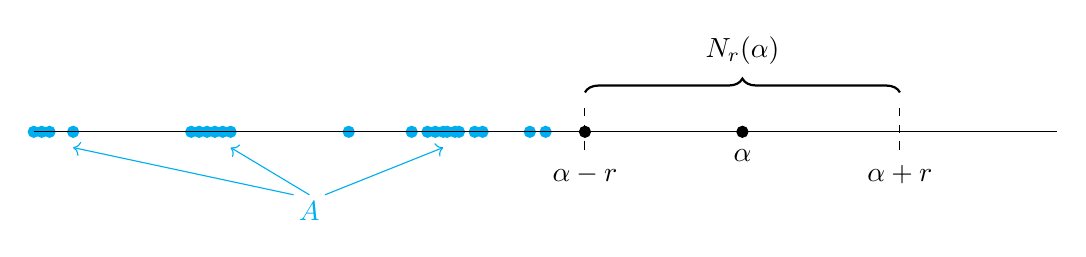
\begin{tikzpicture}
  \centering
    \filldraw[black] (0,0) circle (2pt);
    \filldraw[black] (2,0) circle (2pt) node[below=3pt]{$\alpha $};
    \filldraw[cyan] (-7,0) circle (2pt);
    \filldraw[cyan] (-6.9,0) circle (2pt);
    \filldraw[cyan] (-6.8,0) circle (2pt);
    \filldraw[cyan] (-6.5,0) circle (2pt);
    \filldraw[cyan] (-5,0) circle (2pt);
    \filldraw[cyan] (-4.9,0) circle (2pt);
    \filldraw[cyan] (-4.8,0) circle (2pt);
    \filldraw[cyan] (-4.7,0) circle (2pt);
    \filldraw[cyan] (-4.6,0) circle (2pt);
    \filldraw[cyan] (-4.5,0) circle (2pt);
    \filldraw[cyan] (-3,0) circle (2pt);
    \filldraw[cyan] (-2,0) circle (2pt);
    \filldraw[cyan] (-2.2,0) circle (2pt);
    \filldraw[cyan] (-1.9,0) circle (2pt);
    \filldraw[cyan] (-1.8,0) circle (2pt);
    \filldraw[cyan] (-1.75,0) circle (2pt);
    \filldraw[cyan] (-1.65,0) circle (2pt);
    \filldraw[cyan] (-1.6,0) circle (2pt);
    \filldraw[cyan] (-1.4,0) circle (2pt);
    \filldraw[cyan] (-1.3,0) circle (2pt);
    \filldraw[cyan] (-0.5,0) circle (2pt);
    \filldraw[cyan] (-0.7,0) circle (2pt);
    \draw[cyan] (-3.5,-1) node {$A$};
    \draw[cyan, ->] (-3.7,-0.8) -- (-6.5,-0.2);
    \draw[cyan, ->] (-3.5,-0.8) -- (-4.5,-0.2);
    \draw[cyan, ->] (-3.3,-0.8) -- (-1.8,-0.2);
    \draw (-7,0) -- (6,0);
    \draw [dashed] (4,0.3) -- (4,-0.3) node[align=left,anchor=north]{$\alpha +r$};
    \draw [dashed] (0,0.3) -- (0,-0.3) node[anchor=north]{$\alpha -r$};
    \draw [decorate, decoration = {brace,amplitude=5pt}, thick] (0,0.5) -- (4,0.5) node[midway,yshift=3.5ex]{$N_r(\alpha )$};
    %\draw [decorate,decoration={brace,amplitude=5pt,mirror,raise=4ex}] (1,0) -- (5,0) node[midway,yshift=-3em]{Konvergenzbereich};
\end{tikzpicture}
\end{center}
  \caption{Antagelsen om, at $\alpha $ ikke er et fortætningspunkt fører til modstrid }
\label{fig:sup_fortætning}
\end{figure}


Faktummet, at et fortætningspunkt af en mængde ikke nødvendigvis er et element i mængden (hvilket vi så i eksempel \ref{exa:fortætningspunkter}), motiverer den næste definition.

\begin{definition}[label=def:lukket]{Lukket mængde }{}
  En mængde $A \subseteq \mathbb{R}$ er lukket, hvis den indeholder alle sine fortætningspunkter. 
\end{definition}

Vi vil nu bevise det intuitive resultat, at komplementærmængden til en åben mængde er lukket, og vice versa.
Bemærk, at nogle benytter notationen $\overline A$ til at denotere afslutningen af $A$ (foreningsmængden af $A$ og mængden af alle dens fortætningspunkter), hvor vi her bruger $\overline A$ til at denotere komplementærmængden til $A$.

\begin{theorem}[label=theo:åben_lukket_komp]{Mængde er lukket præcis når dens komplementærmængde er åben}{}
  En mængde $A \in \mathbb{R}$ er lukket hvis og kun hvis dens komplementærmængde $\overline A$ er åben. 
\end{theorem}
\begin{proof} 
  Antag først, at $A$ er lukket.
  Så er alle $x \in \overline A$ ikke fortætningspunkter af $A$, og der eksisterer en omegn $N_r(x)$ sådan at $A \cap N_r(x)=\emptyset$. 
  Det vil sige, at $N_r(x) \subseteq \overline A$, og $x$ er derfor et indre punkt af $\overline A$.
  Således er $A$ åben. 

  Omvendt, antag at $\overline A$ er åben, og lad $p$ være et fortætningspunkt af $A$. 
  Så indeholder alle omegne $N_r(p)$ et punkt $q \in A$, og $p$ er derfor ikke et indre punkt af $\overline A$.
  Siden $\overline A$ er åben, så må $p \in A$.
  Altså indeholder $A$ alle sine fortætningspunkter og må være lukket. 
\end{proof}



\section{Kontinuitet}%
\label{sec:Kontinuitet}
I dette afsnit definerer vi grænseværdien for en funktion stringent med den såkaldte $\varepsilon $-$\delta $-definition.
Vi arbejder dog kun med reele funktioner med delmængder af $\mathbb{R}$ som definitionsmængde. 

Vi undersøger så kontinuerte funktioner med lukkede intervaller som definitionsmængde, da disse funktioner har nogle specielle egenskaber, der ikke er gældende for alle kontinuerte funktioner.
Disse resultater benyttes senere til at bevise vigtige resultater for Riemann-integralet.

\subsection{Grænseværdier af reele funktioner af delmængder af $\mathbb{R}$}%
\label{sub:Grænseværdi}
\begin{definition}[label=def:grænseværdi]{Grænseværdi af funktion}{}
  Antag $X \subseteq \mathbb{R}$, $f:X \to \mathbb{R}$, og $p$ er et fortætningspunkt af $X$.
  Et tal $L$ kaldes for grænseværdien af $f$ i $p$ og vi skriver
  \[
  \lim_{x \to p} f(x)= L,
  \] 
  hvis der for alle $\varepsilon >0$ eksisterer et tal $\delta >0$ sådan at når $x \in X$ og $0<\abs{x-p} < \delta  $, så gælder $\abs{f(x)-L} <\varepsilon $.  
\end{definition}

\begin{figure}[H]
\begin{center}
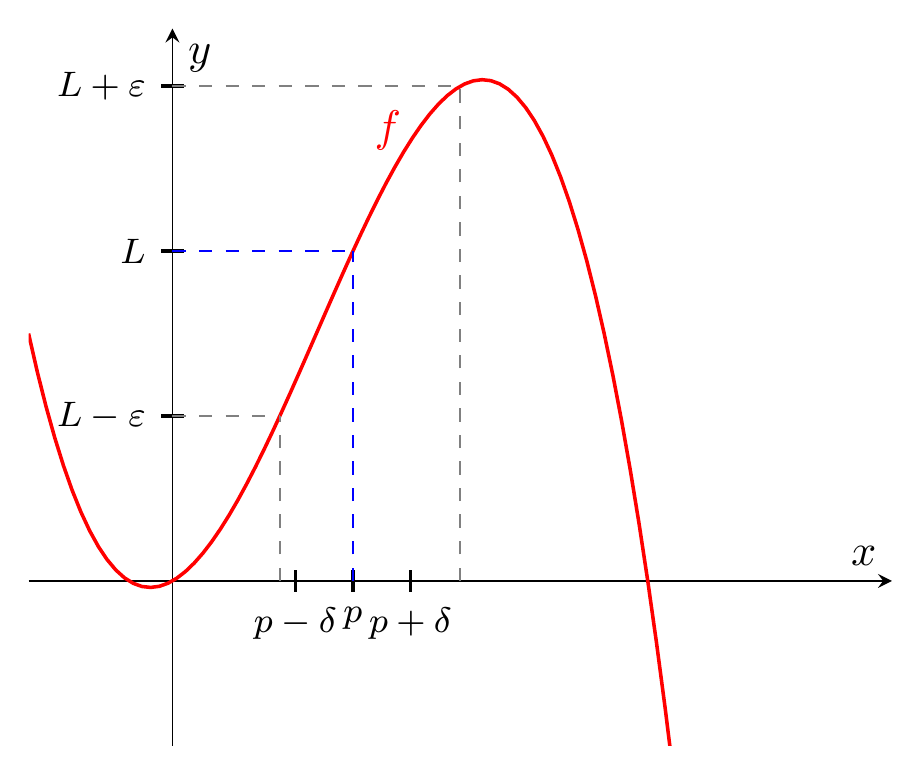
\begin{tikzpicture}[scale=1.6, transform shape]
\begin{axis}[xmin=-1, xmax=5, ymin=-2, ymax=6.7, axis lines=middle,
  xlabel=$x$,ylabel=$y$,
  xtick={0.8541,1.2541,1.6541},
  xticklabels={$p- \delta $, $p$, $p+\delta $},
  xticklabel style={anchor=north, font=\footnotesize},
  ytick={2,4,6},
  yticklabels={$L-\varepsilon $, $L$, $L+\varepsilon $},
  every major tick/.append style={thick, major tick length=5pt, black},
  yticklabel style={anchor=east, font=\footnotesize}
  ]
  \addplot[color=red, domain=-1:5, samples=100, thick]{-x^3 + 3*x^2+x} node[left, pos=0.15] {$f$};
  \draw[color=gray, dashed] (axis cs:0.7459,0) -- (axis cs:0.7459,2);
  \draw[color=gray, dashed] (axis cs:0,2) -- (axis cs:0.7459,2);
  \draw[color=gray, dashed] (axis cs:2,0) -- (axis cs:2,6);
  \draw[color=gray, dashed] (axis cs:0,6) -- (axis cs:2,6);
  \draw[color=blue, dashed] (axis cs:1.2541,0) -- (axis cs:1.2541,4);
  \draw[color=blue, dashed] (axis cs:0,4) -- (axis cs:1.2541,4);
\end{axis}
\end{tikzpicture}
\end{center}
\caption{$\varepsilon $-$\delta $-definition af funktionel grænseværdi}%
\label{fig:epsilondelta}
\end{figure}

Bemærk, at siden $p$ ikke behøver være i definitionsmængden $X$ (se eksempel \ref{exa:fortætningspunkter}), så kan grænseværdien for $f$ sagtens give mening i punkter, hvor selve $f$ ikke er defineret.

\begin{example}[label=exa:grænseværdi]{Grænseværdi i punkt, hvor funktion ikke er defineret}{}
 Lad funktionen $f:\{ x \in \mathbb{R}:x>0 \} \to \mathbb{R}$ være defineret ved
  \[
  f(x)= x^2.
  \] 
  Fra eksempel \ref{exa:fortætningspunkter} har vi, at $0$ er et fortætningspunkt af $\{ x \in \mathbb{R}:x>0 \} $. 
  Vores intuition fortæller os så, at
  \[
  \lim_{x \to 0} f(x)= 0.
  \] 
  Dette vil vi nu bevise stringent via definition \ref{def:grænseværdi}.

  For alle $\varepsilon >0$ vælger vi $\delta =\sqrt{\varepsilon } $. 
  Så har vi, at når $x \in \{ x \in \mathbb{R}:x>0 \} $ og $0<\abs{x-0} =\abs{x} <\delta $, så gælder
  \[
    \abs{f(x)-0} =\abs{x^2}=\abs{x}^2<\delta ^2=\varepsilon.
  \] 
  Altså har vi vist, at $\lim\limits_{x \to 0}f(x)=0$.
\end{example}

Det næste eksempel viser, at selv hvis et punkt $p$ tilhører definitionsmængden af en funktion $f$, så kan vi trods intuitionen godt have $\lim\limits_{x \to p} f(x) \neq f(p)$.

\begin{example}[label=exa:grænseværdi2]{Grænseværdi af funktion i punkt ulig funktionsværdien}{}
  
\end{example}

\subsection{Kontinuerte funktioner på intervaller}%
\label{sub:Kontinuert}


\begin{definition}[label=def:kontinuert]{Kontinuert}{}
 Antag $X \subseteq \mathbb{R}$, $f:X \to \mathbb{R}$ og $p \in X$.

  Så er $f$ kontinuert i $p$, hvis der for alle $\varepsilon >0$ eksisterer $\delta >0$ sådan at når $x \in X$ og $\abs{x-p} < \delta  $, så gælder $\abs{f(x)-f(p)}<\varepsilon $. 

  Hvis $f$ er kontinuert i alle punkter i $X$, så siger vi, at $f$ er kontinuert på $X$. 
\end{definition}

Ved første øjekast ligner dette definitionen af grænseværdier af funktioner til forveksling.
Den største forskel ligger i, at vi her kræver, at $f$ skal være defineret i $p$. 
Tilvarende skal vi i \cref{fig:epsilondelta} blot skrive $f(p)$ i stedet for $L$, for at figuren illustrerer definitionen på kontinuitet. 

Sammenligner vi med definition \ref{def:grænseværdi}, ser vi, at hvis vi også antager, at $p$ er et fortætningspunkt af $X$, så er $f$ kontinuert i $p$ præcis når
\[
\lim_{x \to p} f(x) =f(p).\footnote{Kontinuitet defineres sådan i f.eks. \cite{Brydensholt2018}, s. 34. Bemærk, at grænseværdien $\lim\limits_{x \to p} f(x)$ ikke giver nogen mening, hvis $p$ er et isoleret punkt af $X$.}
\] 
Derudover medfører vores definition, at en funktion er kontinuert i alle isolerede punkter af dens definitionsmængde. 
\begin{example}[label=exa:kontinuert_i_isoleret]{Funktioner er kontinuerte i isolerede punkter af dens definitionsmængde}{}
 Antag $X \subseteq \mathbb{R}$, $f:X \to \mathbb{R}$, og $p$ er et isoleret punkt af $X$. 

  Så er $p$ ikke et fortætningspunkt af $X$, hvilket vil sige, at der eksisterer en omegn $N_r(p)$ sådan at ${N_r(p) \cap X=\{ p \}  }$.
  For alle $\varepsilon >0$ kan vi så vælge $\delta =r$. 
  Så har vi, at når $x \in X$ og $\abs{x-p} <\delta $, så gælder
  \[
  \abs{f(x)-f(p)}=0<\epsilon.
  \] 
  Altså er $f$ kontinuert i $p$. 
\end{example}


\begin{definition}[label=def:begrænset_funktion]{Begrænset funktion}{}
  Antag $X \in \mathbb{R}$.
  Så er en funktion $f:X \to \mathbb{R}$ begrænset, hvis der eksisterer $M \in \mathbb{R}$ sådan at $\abs{f(x)}\leq M$ for alle $x \in X$. 
\end{definition}

Det næste resultat viser, at en kontinuert funktion på et lukket interval er begrænset, og at dens værdimængde i øvrigt også er lukket.

\begin{theorem}[label=theo:kontinuert_begrænset]{Værdimængde for kontinuert funktion på lukket interval er lukket og begrænset}{}
  Hvis en funktion $f:[a;b] \to \mathbb{R}$ er kontinuert, så er $\Vm(f)=\{ f(x):x \in [a;b] \} $ lukket og begrænset.
\end{theorem}

Vi vælger her at udelade beviset, da det falder uden for den indførte teori i denne artikel.\footnote{Sætningen kan bevises via kompakthed og Heine-Borel-sætningen, se \cite{Rudin1976}, s. 40 og 89.
Alternativt kan sætningen også bevises indirekte ved brug af følger og Bolzano-Weierstrass-sætningen, se \cite{Bartle2010}, s. 135.}

\begin{theorem}[label=theo:kontinuert_maks]{Kontinuert funktion på lukket interval har maksimum og minimum}{}
  Antag $f:[a;b] \to \mathbb{R}$ er kontinuert, og lad $\Vm(f)=\{ f(x):x \in [a;b] \} $.
  Så eksisterer $p,\,q \in [a;b]$ sådan at $f(p)=\sup \Vm(f)$ og $f(q)=\inf \Vm(f)$.
\end{theorem}
\begin{proof} 
  
\end{proof}

Bemærk, at uniform kontinuitet også kaldes for ligelig kontinuitet.

\begin{definition}[label=def:uniform_kontinuert]{Uniform kontinuert}{}
  Antag $X \subseteq \mathbb{R}$ og $f:X \to \mathbb{R}$. 
  Så er $f$ uniform kontinuert på $X$ hvis der for alle $\varepsilon >0$ eksisterer $\delta >0$ sådan at der for alle $p,\,q \in X$ gælder
  \[
  \abs{p-q} < \delta \implies \abs{f(p)-f(q)}<\varepsilon .  
  \] 
\end{definition}

Fra definition \ref{def:kontinuert} ser vi, at hvis en funktion $f$ er kontinuert på en delmængde $X \subseteq \mathbb{R}$, så betyder det, at der ved \textit{hvert} punkt $p \in X$ for hver $\varepsilon >0$ kan findes en $\delta >0$ sådan at $\abs{x-p} <\delta $ medfører $\abs{f(x)-f(p)} < \varepsilon  $.
Hvis $f$ derimod er uniform kontinuert på $X$, så eksisterer der for hver $\varepsilon >0$ en $\delta >0$ der opfylder betingelsen for \textit{alle} $p \in X$. 

Definitionen på uniform kontinuitet giver os altså evnen til at kunne skelne mellem, om $\delta $ afhænger af punktet $p$ eller ej. 
Med andre ord er kontinuitet en \textit{nødvendig} betingelse for uniform kontinuitet, hvor uniform kontinuitet er en \textit{tilstrækkelig} betingelse for kontinuitet.
Bemærk også, at en funktion sagtens kan være kontinuert i et \textit{punkt}, hvor uniform kontinuitet kun er defineret på en \textit{mængde}.

Vi vil nu bevise, at hvis en funktion er uniform kontinuert på to lukkede intervaller, så er den uniform kontinuert på foreningsmængden af de to intervaller.

\begin{theorem}[label=theo:uniform_fælles]{Uniform kontinuitet på foreningsmængde af lukkede intervaller, som funktion er uniform kontinuert på}{}
  Antag $f:[a;b]\to \mathbb{R}$, $[c;d] \subseteq [a;b]$, og $[e;f]\subseteq [a;b]$.
  Hvis $f$ er uniform kontinuert på intervallerne $[c;d]$ og $[e;f]$, så er $f$ uniform kontinuert på $[c;d] \cup [e;f]$.
\end{theorem}
\begin{proof} 
  Lad $\varepsilon >0$ være givet. 

  Betragt først tilfældet, hvor $[c;d]\cap [e;f]\neq \emptyset $.
  Siden $f$ er uniform kontinuert på $[c;d]$, har vi, at der eksisterer $\delta _1>0$ sådan at når $p, q \in [c;d]$ og $\abs{p-q} <\delta _2$, så gælder $\abs{f(p)-f(q)} < \frac{\varepsilon }{2} $. 
  Tilsvarende eksisterer $\delta _2>0$, sådan at når $p, q \in [e;f]$ og $\abs{p-q} < \delta _2 $, så gælder $\abs{f(p)-f(q)} <\frac{\varepsilon }{2}$. 
  Lad $\delta =\min (\delta _1, \delta _2)$, og $p, q \in [c;d] \cup [e;f]$.

  \noindent Hvis både $p$ og $q$ er i det samme interval, er det klart, at når $\abs{p-q}<\delta  $, så er $\abs{f(p)-f(q)} <\frac{\varepsilon }{2} < \varepsilon  $. 

  \noindent Hvis vi derimod har, at $p \in [c;d]$ og $q \in [e;f]$ sådan at $p, q \not\in [c;d] \cup [e;f]$, så eksisterer $s \in [c;d] \cap [e;f]$ sådan at når $\abs{p-q} <\delta $, så gælder
  \begin{equation*}
  \begin{split}
 \abs{f(p)-f(q)} &\leq \abs{f(p)-f(s)} + \abs{f(q)-f(s)} \\
  &< \frac{\varepsilon }{2} + \frac{\varepsilon }{2} \\
  &=\varepsilon.
  \end{split}
  \end{equation*}
  Altså er $f$ uniform kontinuert på $[c;d] \cup [e;f]$, hvis $[c;d] \cap [e;f]\neq \emptyset $.

  Antag nu, at $[c;d] \cap [e;f] = \emptyset $.
Siden $f$ er uniform kontinuert på $[c;d]$, eksisterer der $\delta _1>0$ sådan at når $p, q \in [c;d]$ og $\abs{p-q} <\delta _2$, så gælder $\abs{f(p)-f(q)} < \varepsilon$.
Tilsvarende eksisterer $\delta _2>0$, sådan at når $p, q \in [e;f]$ og $\abs{p-q} < \delta _2 $, så gælder $\abs{f(p)-f(q)} <\varepsilon$. 
  Da intervallerne $[c;d]$ og $[e;f]$ er lukkede, så er afstanden mellem dem ikke nul, og der eksisterer $\delta _3>0$, sådan at $\abs{x-y}\geq \delta _3$ for alle $x \in [c;d]$ og $y \in [e;f]$.

  \noindent Lad $\delta = \min (\delta _1, \delta _2, \delta _3)$ og $p, q \in [c;d] \cup [e;f]$.
  Når $\abs{p-q} <\delta $ har vi så, at både $p$ og $q$ må være i enten $[c;d]$ eller $[e;f]$.
  Så gælder $\abs{f(p)-f(q)} <\varepsilon $.
  Altså er $f$ uniform kontinuert på $[c;d] \cup [e;f]$. 


\end{proof}

Det næste resultat viser, at på lukkede intervaller er kontinuerte funktioner også uniform kontinuerte.
Med andre ord er begreberne kontinuitet og uniform kontinuitet altså ækvivalente på lukkede intervaller (husk, at uniform kontinuerte funktioner altid er kontinuerte).

\begin{theorem}[label=theo:kontinuert_uniform]{Kontinuert funktion på lukket interval er uniform kontinuert}{}
  Antag $f:[a;b]\to \mathbb{R}$ er kontinuert. 
  Så er $f$ uniform kontinuert på $[a;b]$.
\end{theorem}
\begin{proof} 
  \footnote{Beviset er delvist baseret på \cite{Clausen1993}, s. 115-116.} 
Lad $\varepsilon >0$ være givet. 
  Siden $f$ er kontinuert i $a$, så eksisterer der $\delta_0$, hvor $0<\delta_0 \leq b$, sådan at når $x \in [a;a+\delta_0 ]$, så gælder $\abs{f(x)-f(a)} < \frac{\varepsilon }{2} $.
  Fra sætning \ref{theo:kontinuert_maks} har vi så, at der eksisterer $\alpha , \beta \in [a;a+\delta_0 ]$, sådan at
  \[
  f(\alpha )=\sup \{ f(x):x \in [a;a+\delta_0 ] \} \text{ og } f(\beta )= \inf \{ f(x):x \in [a;a+\delta_0 ] \}.
  \] 
  For alle $p, q \in [a;a+\delta_0 ]$ har vi så, at
  \begin{equation*}
  \begin{split}
    \abs{f(p)-f(q)} &\leq \abs{f(\alpha )-f(\beta )} \\
    &\leq \abs{f(\alpha )-f(a)} + \abs{f(\beta ) - f(a)} \\
    &<\frac{\varepsilon }{2} + \frac{\varepsilon }{2}\\
    &=\varepsilon.
  \end{split}
  \end{equation*}
  Altså er $f$ uniform kontinuert på $[a;a+\delta_0 ]$.

  Vi har, at $f$ ligeledes er kontinuert i $a + \delta _0$, og med lignende ræsonnement som før, må der så gælde, at der eksisterer $\delta _1$, hvor $0<\delta _1 \leq b-(a+\delta _0)$, sådan at $f$ er uniform kontinuert på $[a+\delta _0-\delta_1;a+\delta_0 + \delta_1]$. 
  Vi påstår, at intervallet $[a;b]$ kan overdækkes med et endeligt antal af disse intervaller. 
  Med andre ord påstår vi, at der eksisterer $\delta _0, \ldots , \delta _n$ sådan, at 
  \[
  [a;b]=[a;a+\delta_0 ] \cup [a+\delta _0-\delta_1;a+\delta_0 + \delta_1] \cup \cdots \cup [a+\delta _0+\cdots +\delta _{n-1}-\delta _n;a+\delta _0+\cdots +\delta _{n}],
  \] 
  hvor $f$ er uniform kontinuert i hvert af intervallerne på højre side af lighedstegnet. 

  Antag nemlig, at $[a;b]$ ikke kan dækkes af endeligt mange af disse intervaller, og lad $U$ være intervallet, som kan overdækkes med et endeligt antal af de beskrevne intervaller, med venstre endepunkt i $a$. 
Så er $U$ ikke tom, og $U$ er opad begrænset med $b$ som overtal. 
  Fra supremum-egenskaben (sætning \ref{theo:supremum-egenskab}) følger det, at $c=\sup U<b$ eksisterer. 
  Imidlertid er $f$ dog kontinuert i $c$, og vi har igen med lignende ræsonnement som før, at der eksisterer $\delta _c>0$ sådan at $f$ er uniform kontinuert i $[c-\delta _c;c+\delta _c]$. 
  Der opstår da modstrid, da vi antog, at $c$ er supremum for $U$. 

Således kan $[a;b]$ overdækkes af et endeligt antal intervaller, hvorpå $f$ er uniform kontinuert.
  Det følger så induktivt fra sætning \ref{theo:uniform_fælles}, at $f$ er uniform kontinuert på $[a;b]$.
\end{proof}



\section{Riemann-integralet}%
\label{sec:Riemann-integralet}
I dette afsnit vil vi definere Riemann-integralet.\footnote{Afsnittet er primært baseret på \cite{Abbott2002}, s. 183-194}
Det skal dog bemærkes, at vi ikke benytter Riemanns originale definition, men derimod en videreudvikling af den franske matematiker Darboux.
Det kan bevises, at de to definitioner på integralet er ækvivalente.\footnote{\cite{Bartle2010}, s. 231-232.}

Vi starter med nogle grundlæggende definitioner, vi har brug for til at definere integralet.
\begin{definition}{Inddeling}{}
  Antag $a,\;b \in \mathbb{R}$ sådan at $a <b$.
  Ved en inddeling $P$ af $[a;b]$ forstår vi en endelig mængde $\{x_0,\dotsc, x_n\}$, hvor
  \[
  a=x_0<x_1<\cdots<x_n=b
  \] 
  og vi skriver 
  \[
  \Delta x_i=x_i-x_{i-1} \quad (i=1,\ldots ,n)
  \]  
\end{definition}
Med en inddeling kan vi dele intervallet $[a;b]$ op i $n$ delintervaller, hvor det $i$'te delinterval har længden $\Delta x_i$:
\[
[a;b]=[x_0;x_1] \cup [x_1;x_2]\cup \cdots \cup [x _{n-1};x_n]
\] 
Vi vil nu definere over- og undersummen af en funktion med hensyn til en given inddeling.

\begin{definition}{Over- og undersum}{}
  Antag $f:[a;b] \to \mathbb{R}$ er en begrænset funktion, og $P=\{x_0,\ldots, x_n\}$ er en inddeling af $[a;b]$. 
  Lad 
  \[
  M_i=\sup \{ f(x):x \in [x _{x_{i-1}};x_i] \} \quad{\text{og}} \quad m_i=\inf \{ f(x):x \in [x _{x_{i-1}};x_i] \}.
  \] 
  Så er oversummen af $f$ med hensyn til $P$ defineret ved
  \[
  U(f,P)=\sum_{i=1}^{n} M_i \Delta x_i.
  \] 
  Tilsvarende er undersummen af $f$ med hensyn til $P$ defineret ved
  \[
  L(f,P)=\sum_{i=1}^{n} m_i \Delta x_i.
  \] 
\end{definition}

Vi kræver i definitionen, at $f(x)$ er begrænset, da vi så fra sætning \ref{theo:supremum-egenskab} ved, at $M_i$ og $m_i$ eksisterer. 

\begin{theorem}[label=theo:ulighed_overundersum]{Uligheder med over- og undersummer}{}
  Antag $f:[a;b] \to \mathbb{R}$ er en begrænset funktion og $P$, $P'$ er inddelinger af $[a;b]$ sådan at $P \subseteq P'$. Så gælder
  \[
  L(f,P)\leq L(f,P') \text{ og }  U(f,P') \leq U(f,P).
  \] 
\end{theorem}
\begin{proof} 
  \footnote{Beviset er baseret på \cite{Axler2020}, s. 3-4.} 
  Lad $P=\{ x_0,\ldots , x_n \} $ og $P'=\{x_0',\ldots x_N'\}$. 
  Siden $P \subseteq P'$, så har vi, at for hver $j=1,\ldots , n$ eksisterer $k \in \{ 0,\ldots , N-1 \} $ og $m \in \mathbb{Z}^+$ sådan at $x _{j-1} =x_k'< \cdots < x _{k+m}'=k_j$.

  Så gælder for hver $i=1, \ldots , m$, at ${\{ f(x):x \in [x'_{k+i-1};x'_{k+i }] \} \subseteq \{ f(x):x \in [x_{j-1},x_j]\}  }$, og 
  \begin{equation*}
  \begin{split}
   m_j&=\inf \{ f(x):x \in [x_{j-1};x_j]\} \\
    &\leq  \inf \{ f(x):x \in [x'_{k+i-1};x'_{k+i }] \}\\
    &=m'_{k+i}.
  \end{split}
  \end{equation*}
Vi får så uligheden 
\begin{equation*}
\begin{split}
  m_j \Delta x_j&=\sum_{i=1}^{m} m_j \Delta x _{k+i}\\
  &\leq \sum_{i=1}^{m} m' _{k+i} \Delta x _{k+i}.
\end{split}
\end{equation*}
  Det følger, at $L(f,P) \leq L(f,P')$. 

  Tilsvarende har vi for hver $i=1,\ldots, m$ også, at
  \begin{equation*}
  \begin{split}
    M_j&=\sup \{ f(x):x \in [x_{j-1};x_j] \} \\
    &\geq \sup \{ f(x):x \in [x'_{k+i-1};x'_{k+i}] \} \\
    &=M'_{k+i},
  \end{split}
  \end{equation*}
  og vi får uligheden
  \begin{equation*}
  \begin{split}
  M_j \Delta x_j&=\sum_{i=1}^{m} M_j \Delta x _{k+i}\\
  &\leq \sum_{i=1}^{m} M' _{k+i} \Delta x _{k+i}.
  \end{split}
  \end{equation*}
  Det følger, at $U(f,P) \geq U(f,P')$
\end{proof}

Beviset for sætning \ref{theo:ulighed_overundersum} kan godt virke uoverskueligt grundet notationen, men \cref{fig:ulighed_overundersum} tydeliggør i høj grad ideen i beviset.

\begin{figure}[H]
\begin{center}
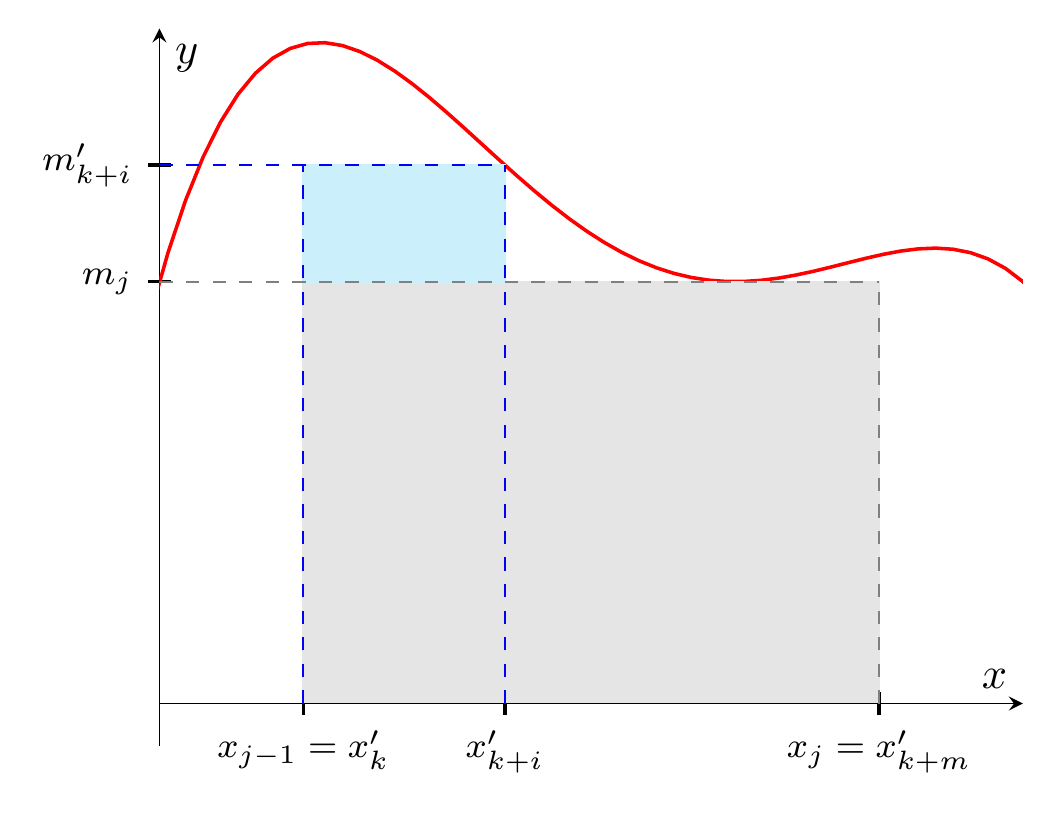
\begin{tikzpicture}[scale=1.6, transform shape]
\begin{axis}[xmin=0, xmax=3, ymin=-0.5, ymax=8, axis lines=middle,
  xlabel=$x$,ylabel=$y$,
  xtick={0.5,1.2,2.5},
  xticklabels={$x _{j-1}=x'_{k}$, $x'_{k+i}$, $x_j=x'_{k+m}$},
  xticklabel style={anchor=north, font=\footnotesize},
  ytick={6.3824,5},
  yticklabels={$m'_{k+i}$, $m_j$},
  every major tick/.append style={thick, major tick length=5pt, black},
  yticklabel style={anchor=east, font=\footnotesize}
  ]
  \addplot[color=red, domain=-1:5, samples=100, thick]{-(x-2)^4 - (x-2)^3 + 2*(x-2)^2+5} node[left, pos=0.15] {$f$};
  \filldraw[gray!20] (axis cs:0.5,0.02) rectangle (axis cs:2.5,5);
  \filldraw[cyan!20] (axis cs:0.5,5) rectangle (axis cs:1.2,6.3824);
  \draw[color=blue, dashed] (axis cs:0.5,0) -- (axis cs:0.5,6.3824);
  \draw[color=blue, dashed] (axis cs:0,6.3824) -- (axis cs:1.2,6.3824);
  \draw[color=gray, dashed] (axis cs:2.5,0) -- (axis cs:2.5,5);
  \draw[color=gray, dashed] (axis cs:0,5) -- (axis cs:2.5,5);
  \draw[color=blue, dashed] (axis cs:1.2,0) -- (axis cs:1.2,6.3824);
\end{axis}
\end{tikzpicture}
\end{center}
  \caption{Ideen i beviset af sætning \ref{theo:ulighed_overundersum}}%
\label{fig:ulighed_overundersum}
\end{figure}



\section{Numerisk integration}%
\label{sec:Numerisk integration}

\section{Diskussion - videreudvikling af integrationsteorien}%
\label{sec:Diskussion}

\section{Konklusion}%
\label{sec:Konklusion}


%%%%%%%%%%%%%%%%%%%%%%% BIBLIOGRAPHY %%%%%%%%%%%%%%%%%%%%%%%

\newpage
\singlespacing %%Makes single spaced
\bibliographystyle{apa-good} %%bib style found in bst folder, in bibtex folder, in texmf folder.
\setlength{\bibsep}{5pt} %%Changes spacing between bib entries
\bibliography{Zotero} %%bib database found in bib folder, in bibtex folder
\thispagestyle{empty} %%Removes page numbers
\end{document}
